\begin{problem}
   This exercise demonstrates how the performance of nearest neighbor degrades as you add more dimensions. Please do the following in a programming language of your choice:

\begin{enumerate}
  \item Generate a “training” dataset with 100~points in 10~dimensions. For 50~of the points, the first dimension ($x_1$) should be~0; for the other~50, the first dimension should be~1. All other dimensions ($x_2$ through $x_{10}$) should be either~0 or~1, selected randomly with equal probability.

  \item Follow the same procedure from step~1 to generate a random ``test'' dataset.

  \item Count the fraction of test points that would be correctly labeled using 1-nearest neighbor with this training data. (One way to do this is by checking if the closest training point to each test point has the same value for the first dimension, $x_1$.) This is the accuracy of nearest neighbor on this synthetic data.

  \item Repeat steps 1--3 10~times, and average the results. This is the average accuracy of nearest neighbor in 10 binary dimensions, with 1 perfectly informative attribute and 9 random ones.

  \item Repeat step~4 with 5, 10, 20, 50, and 100 dimensions. As before, every dimension should be random except for the first ($x_1$). Report the average accuracy for each number of dimensions.
\end{enumerate}

If you're familiar with \texttt{numpy} and Python list comprehensions, it’s possible to do this exercise with just 30~lines of well-structured code. If you do everything from scratch or use a more verbose language, it’s a few more lines of code but it still shouldn't be too difficult.

For your answer to this question: please include:

\begin{enumerate}[(a)]
  \item the average accuracies obtained in step~5,
  \item a graph showing the accuracy versus the number of dimensions, and
  \item a printout of the code you used to help answer this question. (Your code must be your own work.)
\end{enumerate}
\end{problem}

The average accuracies are reported in Table~\ref{tab:P02:EffectAccuracy} while the graph of the results are included in Figure~\ref{fig:P02:KnnDimensionPlot}.

\begin{table}[h]
  \centering
  \caption{Problem~\#2: Effect of dimension on 1-NN accuracy}\label{tab:P02:EffectAccuracy}
  \begin{tabular}{|c|c|}
    \hline
    Dimension & 1-NN Accuracy \\\hline\hline
    1   & 1.000  \\\hline
    % 2   & 1.000  \\\hline
    % 3   & 1.000  \\\hline
    % 4   & 1.000  \\\hline
    5   & 0.989  \\\hline
    10  & 0.848  \\\hline
    20  & 0.760  \\\hline
    50  & 0.670  \\\hline
    100 & 0.617  \\\hline
  \end{tabular}
\end{table}

\begin{figure}[h]
  \centering
  \centering
\begin{tikzpicture}[
  ]
  \pgfplotstableread[col sep=comma] {plots/p02_data.csv}\pData
  \begin{axis}[
      width=10cm,
      height=10cm,
      xmin=0,
      xmax=100,
      minor x tick num=10,
      ymin=0.5,
      ymax=1,
      minor y tick num=5,
      every tick label/.append style={font=\scriptsize},  % Reduce axis font size
      xlabel={$d$},
      ylabel={Accuracy},
      xlabel style={font=\scriptsize},
      ylabel style={font=\scriptsize},
      ylabel shift = -4pt,
      title={Problem~\#2: Effect of Dimension of $x$ on KNN Accuracy},
    ]
    \addplot[color=blue, thick] table[x index=0,y index=1] {\pData};
  \end{axis}
\end{tikzpicture}

  \caption{Effect of dimension on 1-NN accuracy}\label{fig:P02:KnnDimensionPlot}
\end{figure}

\FloatBarrier
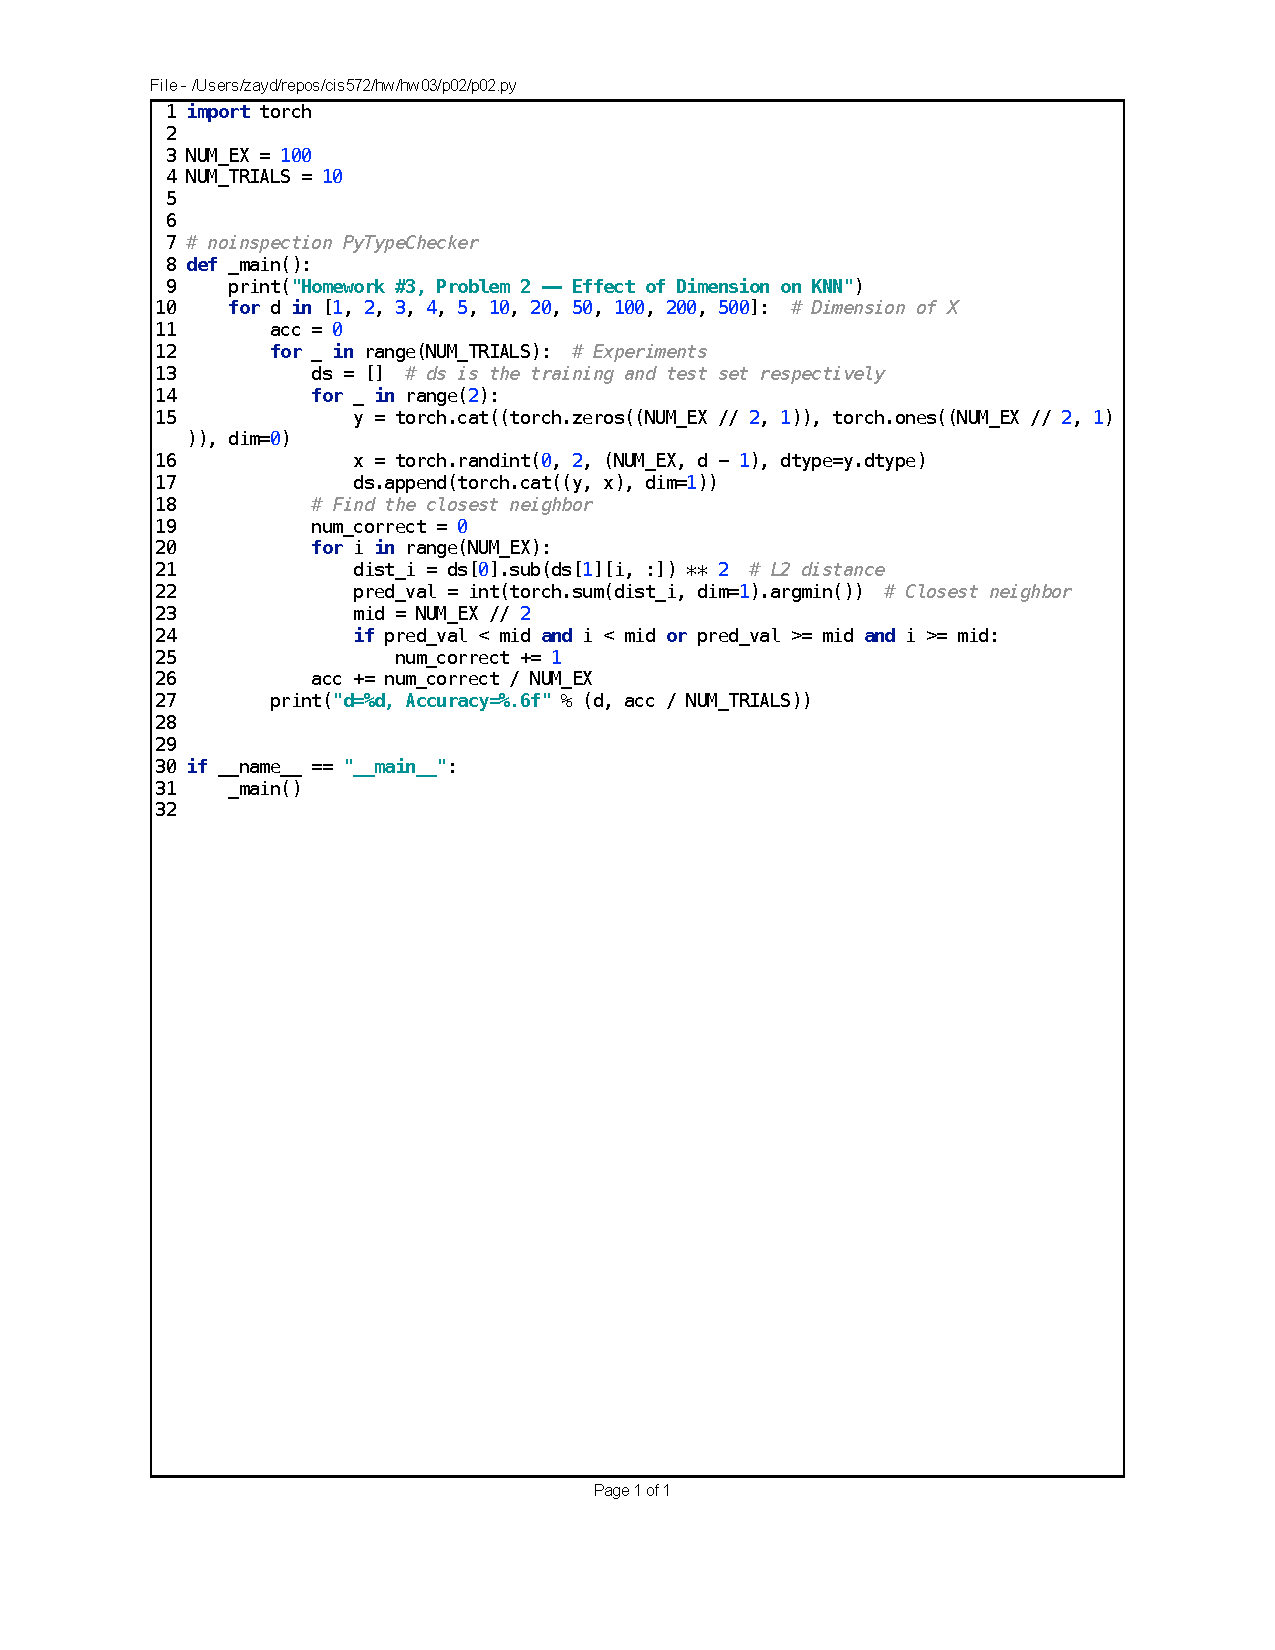
\includepdf[pages=-]{pdf/p02_src.pdf}
